% vim: set tw=0:
\documentclass{beamer}
\usepackage{graphicx}

% Reasonable themes:
% Antibes Bergen Berkeley Berlin Frankfurt Goettingen Ilmenau Luebeck Malmoe
% Montpellier PaloAlto Rochester Singapore Szeged Warsaw bars boxes
% compatibility default lined plain shadow sidebar split tree
% And these ones include the author's name on every slide:
% Berkeley

% Declare themes.
\mode<presentation>
\usetheme{UWHEP}

% Personal macros.
\newcommand{\email}[1]{{\texttt #1}}
\newcommand{\newframe}[1]{\section{#1}
    \frametitle{\sc{#1}}}
\newcommand{\subframe}[1]{\subsection{#1}
    \frametitle{\sc{#1}}}
\newcommand{\supers}[1]{\ensuremath{^\textrm{#1}}}
\newcommand{\subs}[1]{\ensuremath{_\textrm{#1}}}
\newcommand{\ca}{\ensuremath{\sim}}

% Author information.
\title[Collaborative Development]{Collaborative Development at USCMS Tier2s}
\author[Maier, Thomas]{
    Will Maier\inst{1} \and Michael Thomas\inst{2}\\ 
    {\tt wcmaier@hep.wisc.edu}\\
    {\tt thomas@hep.caltech.edu}}
\institute[UW, CIT]{
    \inst{1}University of Wisconsin
    \and
    \inst{2}Caltech}
\date{\today}
\logo{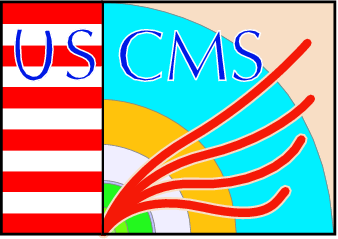
\includegraphics[height=0.6cm]{../../../Graphics/USCMS_logo.png}}
%\logo{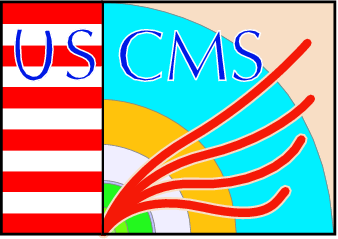
\includegraphics[height=0.6cm]{../../../Graphics/USCMS_logo.png}\hspace{.1cm}
\includegraphics[height=0.75cm]{../../../Graphics/UW_logo.png}}

\begin{document}

\begin{frame}
    \titlepage
\end{frame}

%\section{Overview}
%\begin{frame}
%    \tableofcontents
%\end{frame}

\begin{frame}
\frametitle{Problem and Proposal}
Today\ldots{}
\begin{itemize}
    \item Sites develop scripts and configurations separately
    \item University of Foo can't easily compare or integrate their work with that from Bar Institute of Technology
    \item Solutions to common problems diverge or are reimplemented in isolation
\end{itemize}
But what if we had a common collection and integration point for the work we currently do at our sites?
\end{frame}

\begin{frame}
\frametitle{How it might look}
\begin{itemize}
    \item A simple shared repository made available through a commonly agreed version control system
    \item Separate subdirectories/subrepositories for each site
    \item One shared subdirectory/subrepository for common and integrated work
    \item Parallel (but public) work continues on site-specific and unintegrated code
    \item As time permits, interested folks work together to integrate site work in the common area
    \item As often as is possible, new site or common contributions should have basic documentation
\end{itemize}
\end{frame}

\begin{frame}
\frametitle{Details\ldots{}}
\begin{itemize}
    \item Usefulness of the repository scales with participation
    \begin{itemize}
        \item Can we commit to moving existing scripts and maintenance into something like this?
    \end{itemize}
    \item Would you use such a thing?
    \begin{itemize}
        \item What would make you more likely to use it?
    \end{itemize}
    \item What version control system should we use?
    \begin{itemize}
        \item Obvious options include CVS, SVN, git, hg, \ldots{}
        \item Barrier to entry should be low
    \end{itemize}
    \item CIT or Wisconsin (or you?) can host
\end{itemize}
\end{frame}

\end{document}
